\chapter{Ergebnis und Ausblick}

Das Ziel dieser Arbeit war es, einen rudimentären Prototyp einer TD testgetrieben zu entwickeln. In diesem Kapitel möchten wir nun unser Ergebnis vorstellen und einen Ausblick geben, wie man mit dieser Code-Basis weiter verfahren könnte.

Zunächst möchten wir einige Bilder des Prototyps zeigen, in denen die Spielwelt dargestellt ist.\\

\begin{figure}[h]
\centering
\includegraphics[width=1\linewidth]{./images/Kapitel_Ergebnis_und_Ausblick/Aufbau_der_Szene}
\caption[Aufbau der Spielwelt]{Aufbau der Spielwelt}
\label{fig:Aufbau_der_Szene}
\end{figure}

Wie man sieht, orientiert sich die Spielwelt stark an dem schematischen Aufbau aus \autoref{fig:Schematischer_Aufbau_der_Szene} auf Seite \pageref{fig:Schematischer_Aufbau_der_Szene}. Der weiße Block links im Bild stellt das Hauptgebäude des Spielers dar, welches es zu verteidigen gilt. In der Mitte steht eine Verteidigungsanlage und die Gegner laufen auf dem steinigen Weg von rechts nach links.
\pagebreak

Die nachfolgenden Bilder zeigen, wie auf die Gegner geschossen wird. Dabei fliegen kleine Kugeln auf einer parabolischen Flugbahn auf den Gegner, der durch eine größere Kugel dargestellt wird. Über dem Gegner ist ein Lebensbalken zu sehen, der seine verbleibenden Lebenspunkte mit der Breite des grünen Streifens repräsentiert.\\

\begin{figure}[h]
\centering
\includegraphics[width=0.9\linewidth]{./images/Kapitel_Ergebnis_und_Ausblick/Tower_schiesst_1}
\caption[Turm schießt auf Gegner]{Turm schießt auf Gegner\\Der Lebensbalken des Gegners ist voll.}
\label{fig:Tower_schiesst_1}
\end{figure}

\begin{figure}[h]
\centering
\includegraphics[width=0.9\linewidth]{./images/Kapitel_Ergebnis_und_Ausblick/Tower_schiesst_2}
\caption[Turm schießt auf Gegner]{Turm schießt auf Gegner\\Der Gegner wurde geschädigt, wie man an seinem Lebensbalken sehen kann.}
\label{fig:Tower_schiesst_2}
\end{figure}

Die Gegner erscheinen alle 5 Sekunden auf der rechten Seite und werden vom Turm beschossen, sobald sie in seiner Reichweite sind. Stirbt ein Gegner, sucht sich der Turm ein neues Ziel. Dies wiederholt sich solange, bis der Spieler das Programm beendet. An dieser recht einfachen Szene ist noch die Umsetzung des Turms erwähnenswert. Dieser besteht nicht nur aus einem \textit{GameObject}, sondern enthält neben dem Objekt für das Model auch noch zwei weitere \textit{GameObjects}. Das eine haben wir \textit{ProjectileSpawner} genannt, dessen Position als Abschusspunkt für die Projektile dient. Andernfalls würden diese am Boden des Turms starten. Außerdem kann man dadurch den Startpunkt je nach Turm-Model variieren, ohne das Skript verändern zu müssen.\\
Das Zweite soll erkennen sobald ein Gegner in Reichweite kommt oder diese wieder verlässt. Dafür haben wir ein leeres \textit{GameObject}, welches zu dem Turm dazugehört, einen sogenannten \textit{Collider} gegeben. Dieser registriert Berührungen mit anderen \textit{GameObjects} und löst eine Methode in einem angehängten Skript aus. Wie das genau funktioniert wird weiter unten erläutert. Die Größe des \textit{Colliders} wird nun an die Reichweite des Turms angepasst.\\
In dem nachfolgenden Bild sieht man diesen als grüne Sphäre um den Turm. Im Spiel ist diese natürlich nicht zu sehen. Die Kugelform gewährleistet, dass auch fliegende Gegner erst angegriffen werden, wenn sie sich wirklich in Reichweite befinden. Möchte man dies nicht, sollte man einen zylinderförmigen \textit{Collider} verwenden.\\

\begin{figure}[h]
\centering
\includegraphics[width=0.8\linewidth]{./images/Kapitel_Ergebnis_und_Ausblick/Tower_RangeCollider}
\caption[\textit{RangeCollider} des Turms]{\textit{RangeCollider} des Turms\\Repräsentiert die Reichweite des Turms und erkennt wenn Gegner eintreten, beziehungsweise diese wieder verlassen.}
\label{fig:Tower_RangeCollider}
\end{figure}
\clearpage 

Als nächstes möchten wir das Ergebnis mit unserer, in \autoref{sec:Konzept} definierten, Grobstruktur vergleichen. Eine Abbildung des Klassendiagrammes des Ergebnisses befindet sich auf der nächsten Seite. Zur besseren Lesbarkeit wird auch die Grobstruktur nochmals aufgeführt und es wird auf Methoden und Attribute verzichtet. Die farbliche Strukturierung der \textbf{\textcolor{ScriptClass}{Skripte}} und der \textbf{\textcolor{ScriptLogicInterface}{Logik-Skript-Schnittstellen}} bleibt erhalten. Die \textbf{\textcolor{LogicClass}{Logik}} wurde allerdings in Klassen unterteilt die für \textbf{\textcolor{HealthClass}{Lebenspunkte}}, \textbf{\textcolor{MovementClass}{Bewegungen}} beziehungsweise \textbf{\textcolor{AttackClass}{Angriffe}} und \textbf{\textcolor{AttackClass}{Schaden}} verantwortlich sind.\\

\begin{figure}[h]
\centering
\includegraphics[width=1\textwidth]{./images/Kapitel_Ergebnis_und_Ausblick/Grobstruktur}
\caption{Grobstruktur aus \autoref{sec:Konzept} \nameref{sec:Konzept}}
\label{fig:Grobstruktur_Ergebnis}
\end{figure}
	
\begin{figure}[h]
\centering
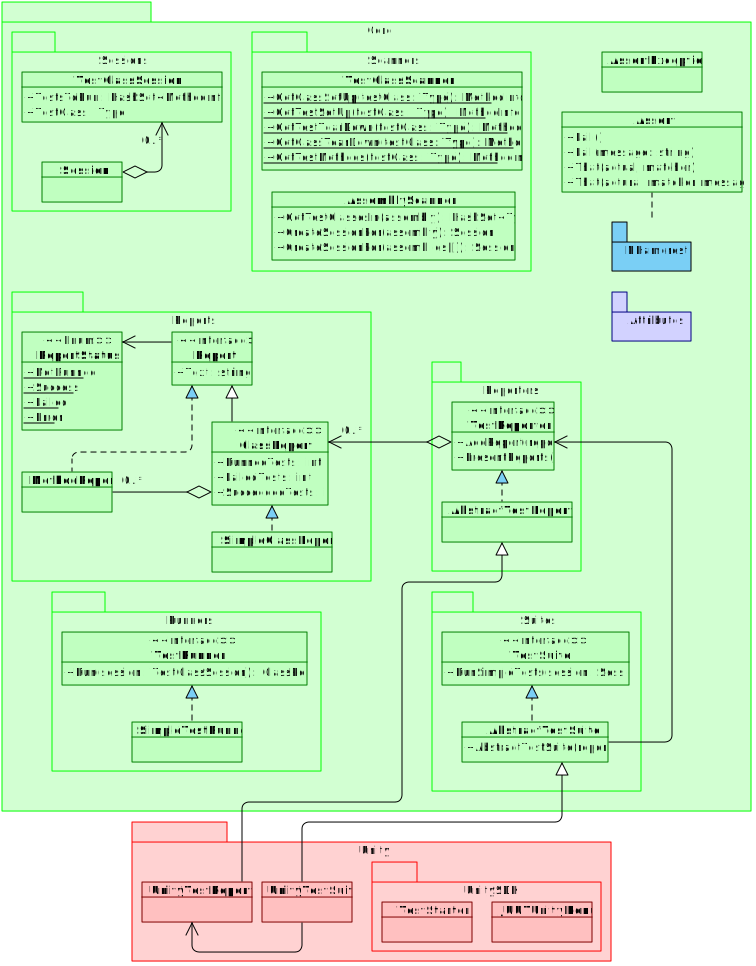
\includegraphics[width=1\textwidth]{./images/Kapitel_Ergebnis_und_Ausblick/Overview}
\caption{Klassendiagramm des Ergebnisses}
\label{fig:Overview}
\end{figure}
\clearpage

Im Großen und Ganzen lagen wir mit unserem Konzept richtig. So mussten wir keine Klassen entfernen, sondern es wurden lediglich neue hinzugefügt, die wir während der Planung nicht berücksichtigt haben. Dazu gehören die Enumerationen \textit{ArmorType} und \textit{DamageType}, welche die unterschiedlichen Schadens- und Rüstungstypen repräsentieren, sowie die Klasse \textit{TargetStrategy}. Diese gehört einem Turm und wählt aus einer Menge von Gegnern das nächste Ziel, das angegriffen werden soll.\\
Auch bei den \textbf{\textcolor{ScriptClass}{Skripten}} kamen weitere hinzu. Erwähnenswert ist hierbei das \textit{RangeColliderScript}, welches einen Turm referenziert und die Gegner verwaltet, die sich in dessen Reichweite befinden. Sobald ein Gegner in die Reichweite des Turmes kommt, löst dies die \textit{OnCollisionEnter}-Methode des Skripts aus. Diese überprüft ob das kollidierte Objekt ein Gegner ist und fügt ihn gegebenenfalls zu der Menge der Ziele des Turms hinzu. Das Entfernen eines Gegners funktioniert genau so, nur wird hier die \textit{OnCollisionExit}-Methode verwendet.
\\
\begin{lstlisting}[caption={[\textit{OnCollisionEnter}-Methode des \textit{RangeColliderScripts}]\textit{OnCollisionEnter}-Methode des \textit{RangeColliderScripts}}]
private void OnCollisionEnter(Collision collision) {
	var creepScript = collision.gameObject.GetComponent<CreepScript>();
	if (creepScript != null) {
		Unit unit = creepScript.Creep;
		Tower.AddUnitInRange(unit);
	}
}
\end{lstlisting}

Eine weitere oft eingesetzte Anpassung, war die Unterteilung der Funktionalitäten in unterschiedliche Unterklassen. So gibt es nun neben einer abstrakten Oberklasse \textit{Attack} noch die Unterklassen \textit{PointTargetAttack}, \textit{UnitSeekingAttack} und \textit{PredictionAttack}. Diese unterscheiden sich in der Art und Weise, wie das Projektil auf das Ziel zufliegt.

So fliegen die Projektile von \textit{PointTargetAttack} einfach auf den Zielpunkt zu, was zum Beispiel bei Katapulten verwendet werden könnte. \textit{UnitSeekingAttack} erzeugt Projektile, die dem Ziel nachfliegen und somit auf jeden Fall treffen. Dies könnte bei magischen Geschossen oder zielsuchenden Raketen eingesetzt werden. Der verbleibende Angriff ist so ähnlich wie die \textit{PointTargetAttack}, nur  berechnet sie vor dem Schuss den Schnittpunkt zwischen dem Gegner und dem Projektil, sodass das Ziel auch getroffen wird, wenn es sich bewegt. Zur Zeit ist dies so implementiert, dass der Angriff auf jeden Fall trifft. In Zukunft könnte man hier eine Ungenauigkeit einbauen, um das Spiel realistischer zu machen. Die Oberklasse übernimmt dabei verwaltende Aufgaben. Zum Beispiel, um zu überprüfen ob die Attacke wieder schießen darf und die Auswahl des aktuellen Zieles (über die \textit{TargetStrategy} des Turms).\\
Dieses Prinzip der Unterteilung wurde auch verwendet um unterschiedliche Bewegungsformen, wie zum Beispiel lineare und parabolische Flugbahnen, zu realisieren und für verschiedene Arten das nächste Ziel eines Turms auszuwählen. Die Verwendung dieser Objekte erfolgt immer über die Oberklasse. So hat der Turm zum Beispiel ein Attribut vom Typ \textit{Attack}, sodass man sein Verhalten zur Laufzeit ändern kann, ohne ein komplett neues Turm-Objekt zu erzeugen. Dies könnte beim Aufbessern eines Turmes verwendet werden.

Getestet wird unser Programm von zehn Testklassen mit insgesamt 38 Testmethoden. Durch die hohe Testabdeckung ist die Spiellogik robust gegenüber Fehlern bei Änderungen. Was sich, auf Grund der fehlenden Unterstützung durch die Frameworks, nicht automatisch testen lässt sind die Skripte, weswegen wir auch versucht haben den Großteil der Logik unabhängig vom Skript zu machen. Dies ist uns gut gelungen, denn wenn man sich von Visual Studio die Code-Metriken berechnen lässt sieht man, dass von 485 Zeilen Produktivcode nur 81 in den Skripten stehen. So ist das Skript für die Projektile nur wenige Zeilen lang und auch das Skript für den Turm, welches etwas länger ist, enthält kaum Logik, sondern nur Unity spezifischen Code, um zum Beispiel die \textit{GameObjects} für die Projektile zu erzeugen oder um den \textit{Collider} an der Angriffsreichweite anzupassen.\\
Allerdings lassen sich manche wichtigen Dinge nicht testen. Zum Beispiel ob ein Gegner auch erkannt wird, wenn er in die Reichweite eines Turmes kommt, ob sich der Turm auch an die Angriffsgeschwindigkeit hält oder ob sich ein Gegner nach dem Treffer von einem Projektil auch korrekt verhält. Diese Verhalten sind zwar in der Spiellogik definiert und auch getestet, allerdings müssen sie von den Skripten korrekt weitergeleitet und angewendet werden.\\
Außerdem ist in unserem Prototypen noch keinerlei Benutzerinteraktion implementiert. Diese kann man auch nur in geringem Maße in die Spiellogik auslagern und würde somit ungetestet bleiben.

In der Zukunft könnte der Prototyp erweitert und zu einem richtigen Spiel werden. Dafür bräuchte es zum Beispiel eine gewisse Benutzerinteraktion und typische Spielelemente, die das Spielen erst spielenswert machen. Dazu gehört ein Punkte-, oder Belohnungssystem, was mit dem Erhalt von Geld realisiert werden kann. Mit diesem Geld könnte man Updates, neue Türme, oder sonstige Verbesserungen kaufen. In der Spielelogik fehlt also noch der Benutzer und sein Status.\\
Zusätzlich muss eine richtige Spielwelt realisiert werden. Bei einer Tower Defense könnte diese auch prozedural erzeugt sein, so dass die einzelnen Levels immer neu generiert und aus vorhandenen Bausteinen zusammengesetzt werden. Diese Generierung könnte ebenfalls in der Spielelogik Platz finden. 

Was für ein richtiges Spiel ebenso fehlt, sind die 3D-Modelle. Wir haben uns in dem Prototypen nur auf den Code hinter dem Spiel gekümmert, deswegen ist von Modellen nicht viel zu sehen. Außer einem Turm, der versuchsweise in Autodesks 3ds Max erstellt und in Unity eingebunden wurde. Auch hier ist einiges prozedural möglich, sodass kleine Bausteine in 3D-Modellierungsprogrammen erstellt werden, die von einer Spielelogik zur Laufzeit in ein größeres Modell zusammengebaut werden. Im Extremfall können so ausgefallene Gegner entstehen, wie zum Beispiel böse Roboter in einem futuristischen Setting, oder Aliens mit wechselnden Gliedmaßen. Aber auch Türme könnten prozedural entstehen, da die Grundform fest steht und die einzelnen Teile variieren können. So könnten Spieleelemente nicht nur prozedural erstellt, sondern vom Benutzer auf Wunsch zusammengebaut werden.

Der gesamte Sourcecode befindet sich in einem \textit{git}-Repository auf github.com, das unter \url{https://github.com/JonasGoldt/TDGD\_TD/} erreichbar ist. Hier befindet sich auch eine komplilierte Version unseres Prototyps.